\documentclass[text05.tex]{subfiles}
\begin{document}
\section{FaBoの\ruby{接続}{せつ|ぞく}}
この\ruby{授業}{じゅ|ぎょう}ではFaBoのシールドとFaBoのブリックを使います。FaBoはセンサーとRaspberry Piを\ruby{簡単}{かん|たん}につなぐことができるよう、あらかじめ配線がされています。
\begin{center}
  \begin{minipage}[b]{0.45\linewidth}
    \begin{figure}[H]
      \centering
      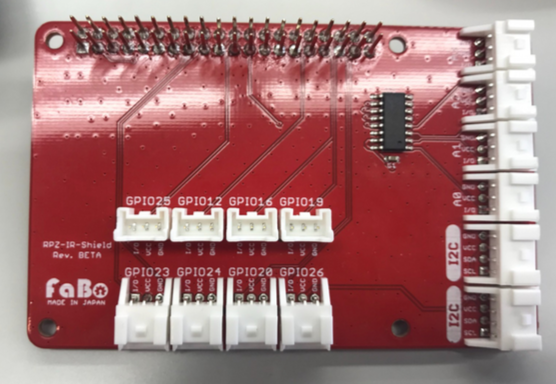
\includegraphics[keepaspectratio, scale=0.6]{../../asset/image/text05-img004.png}
      \caption{Faboのシールド}
      \label{fig4}
    \end{figure}
  \end{minipage}
  \begin{minipage}[b]{0.45\linewidth}
    \begin{figure}[H]
      \centering
      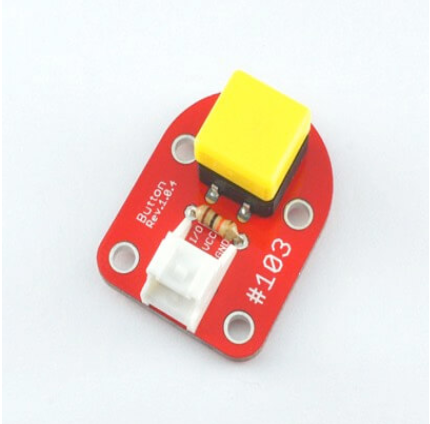
\includegraphics[keepaspectratio, scale=0.6]{../../asset/image/text05-img005.png}
      \caption{Faboのブリック}
      \label{fig5}
    \end{figure}
  \end{minipage}
\end{center}
LEDは電池で動きますが、FaBoブリックはRaspberry Piを\ruby{電源}{でん|げん}として動きます。FaBoでないセンサーは、\ruby{電源}{でん|げん}のプラスとマイナス、センサーの出力などを考えて、Raspberry Piに\ruby{繋}{つな}ぎます。しかし、FaBoのシールドとブリックは必要な配線が\ruby{統一}{とう|いつ}されているため、自分でどのように線を\ruby{繋}{つな}ぐかを考えなくても\ruby{簡単}{かん|たん}に使えます。
それでは、早速FaBoを使ってみましょう。

\begin{itembox}[c]{\Large\textcolor{red}{注意！}}
  FaBoのシールドをRaspberry Piとつなげるときは、必ずRaspberry Piをシャットダウンして\ruby{電源}{でん|げん}を切りましょう。
\end{itembox}

\subsection{Raspberry PiとFaBoブリックの\ruby{接続}{せつ|ぞく}}
\begin{enumerate}
  \item Raspberry Piの\ruby{電源}{でん|げん}を切ります。\\
  \item ケーブルを使用して、FaBoのシールドをRaspberry Piとつなげます。この時、なるべくシールドをまっすぐに\ruby{押}{お}しこむようにしましょう。ピン（\ruby{金属}{きん|ぞく}の\ruby{棒}{ぼう}の部分）を曲げないように注意してください。シールドにもトゲのある所があるのでケガをしないように注意しましょう。\\
  \begin{minipage}[b]{0.4\linewidth}
    \begin{figure}[H]
      \centering
      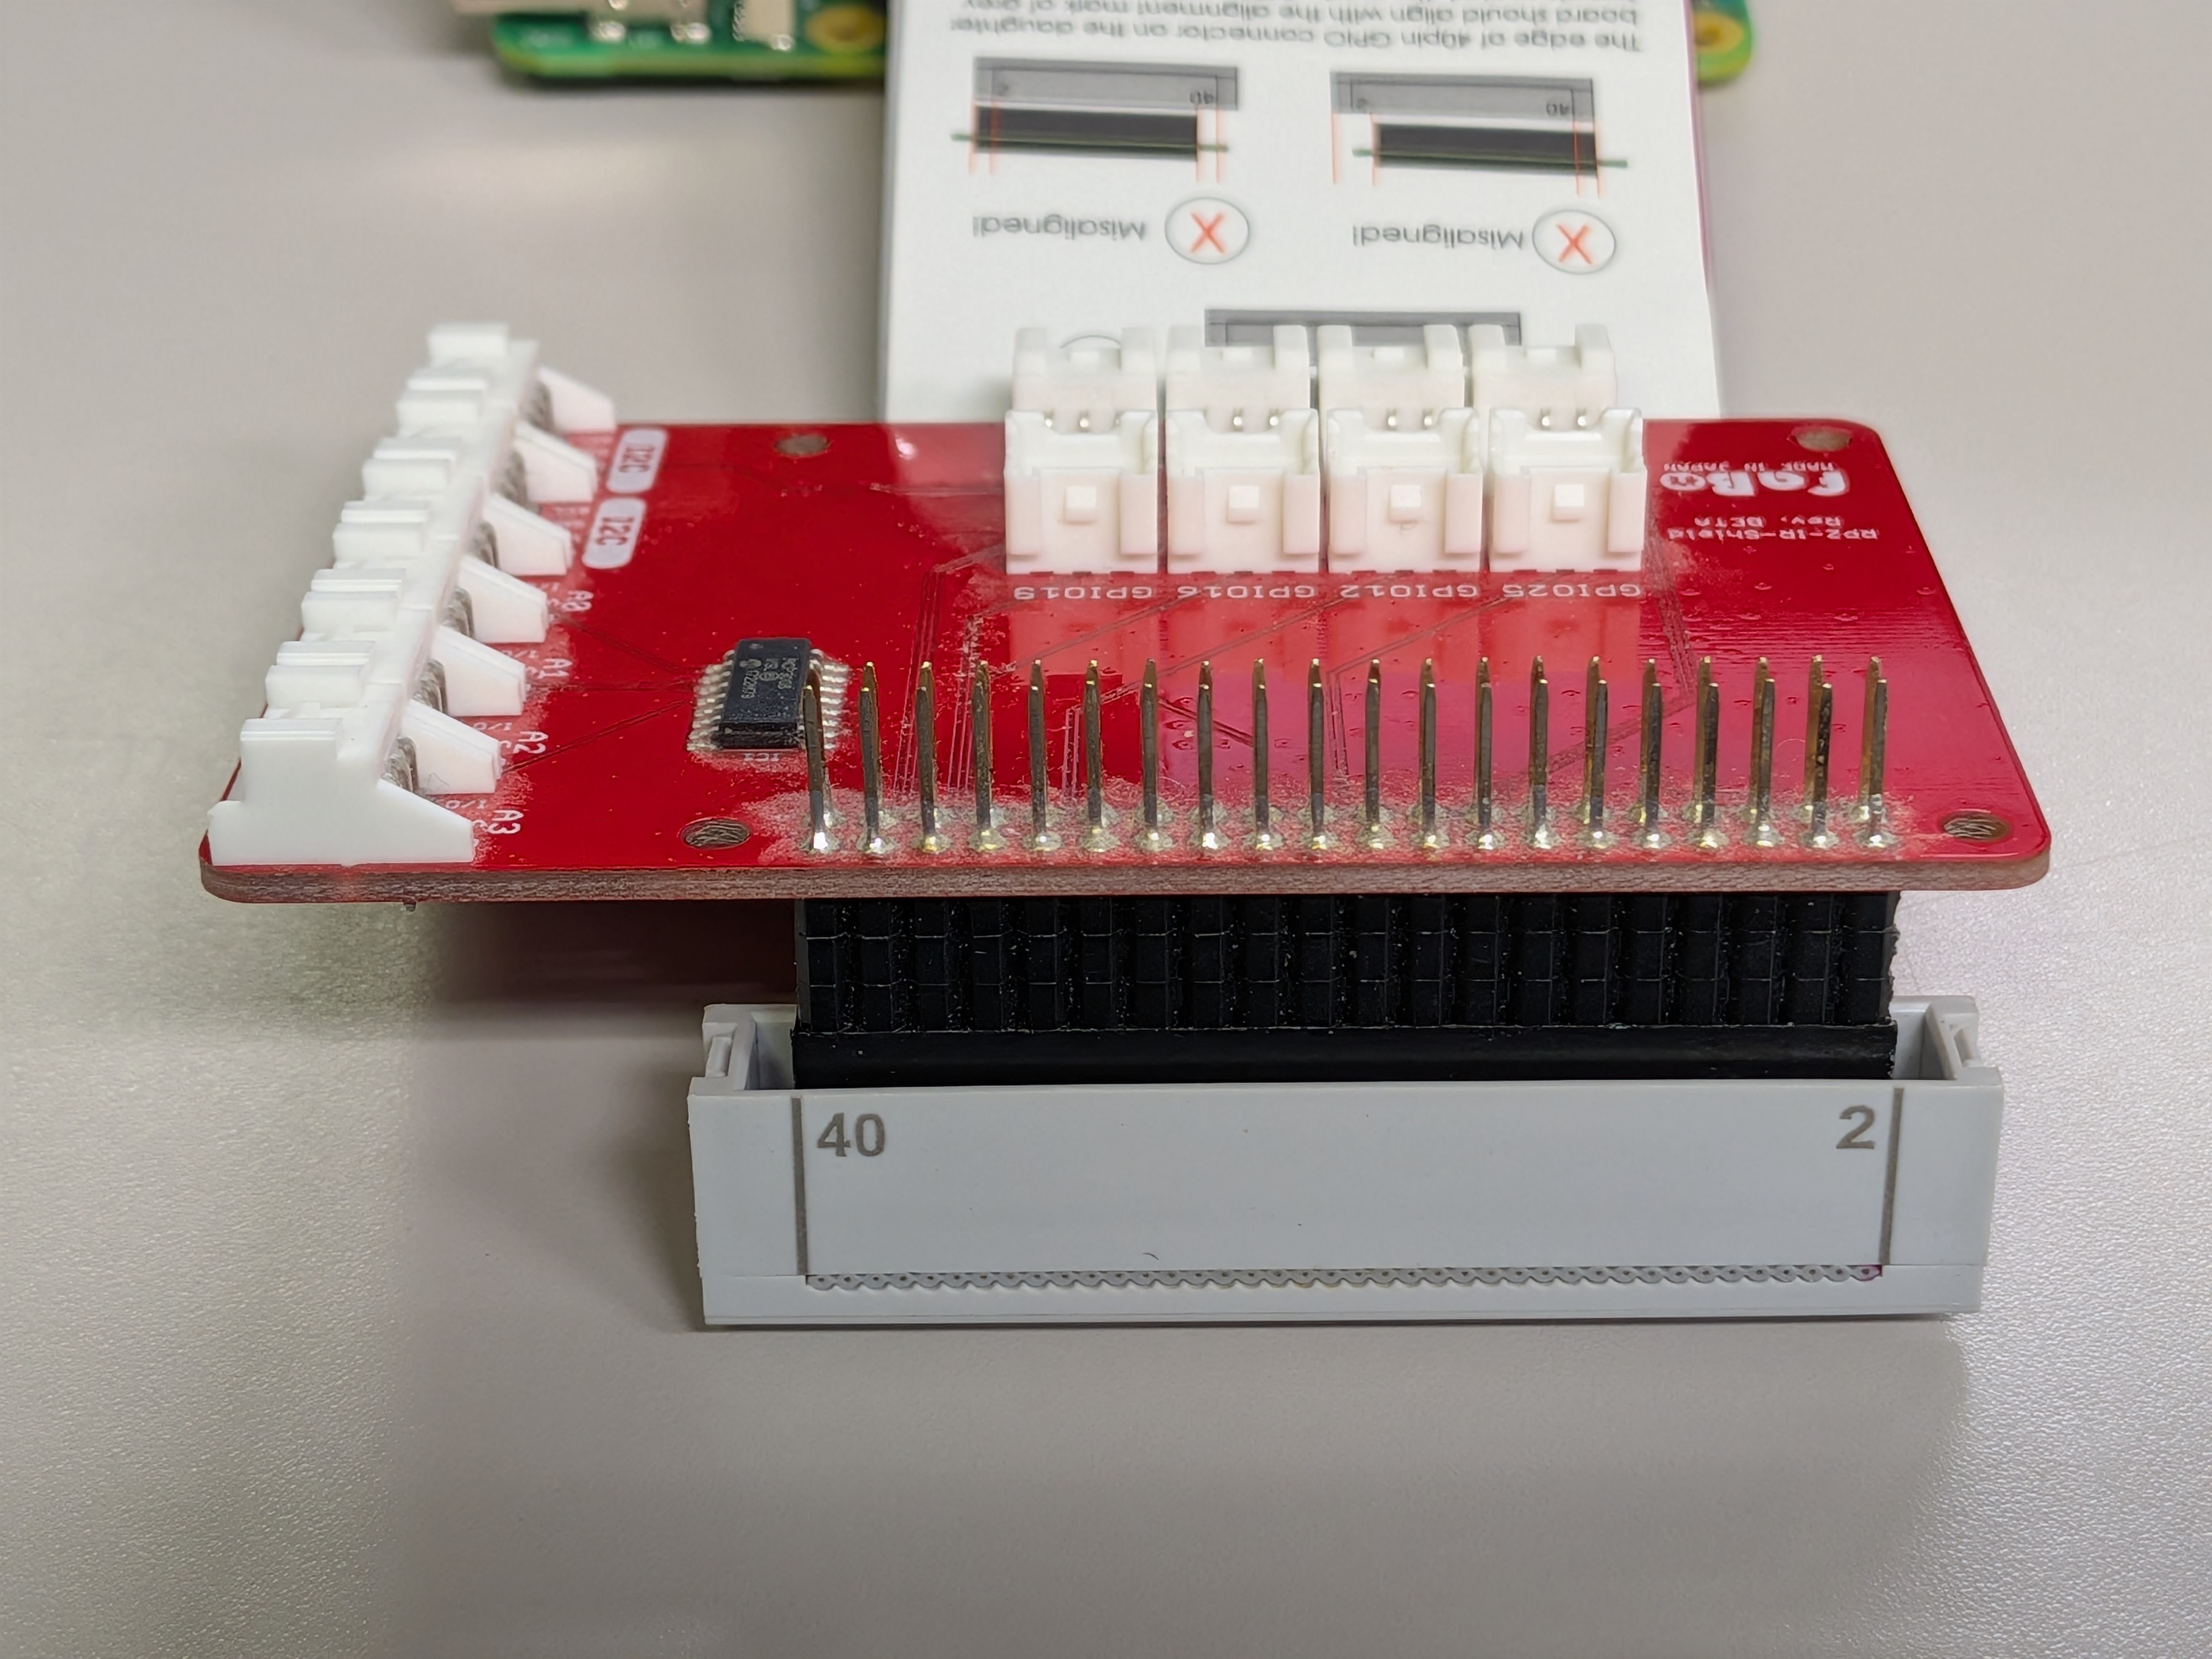
\includegraphics[width=.8\hsize]{../../asset/image/fabo_and_cable_rearview.jpg}
      \caption{FaBoのシールドとケーブルの\ruby{接続}{せつ|ぞく} (後ろから見た図)}
    \end{figure}
  \end{minipage}
  \begin{minipage}[b]{0.4\linewidth}
    \begin{figure}[H]
      \centering
      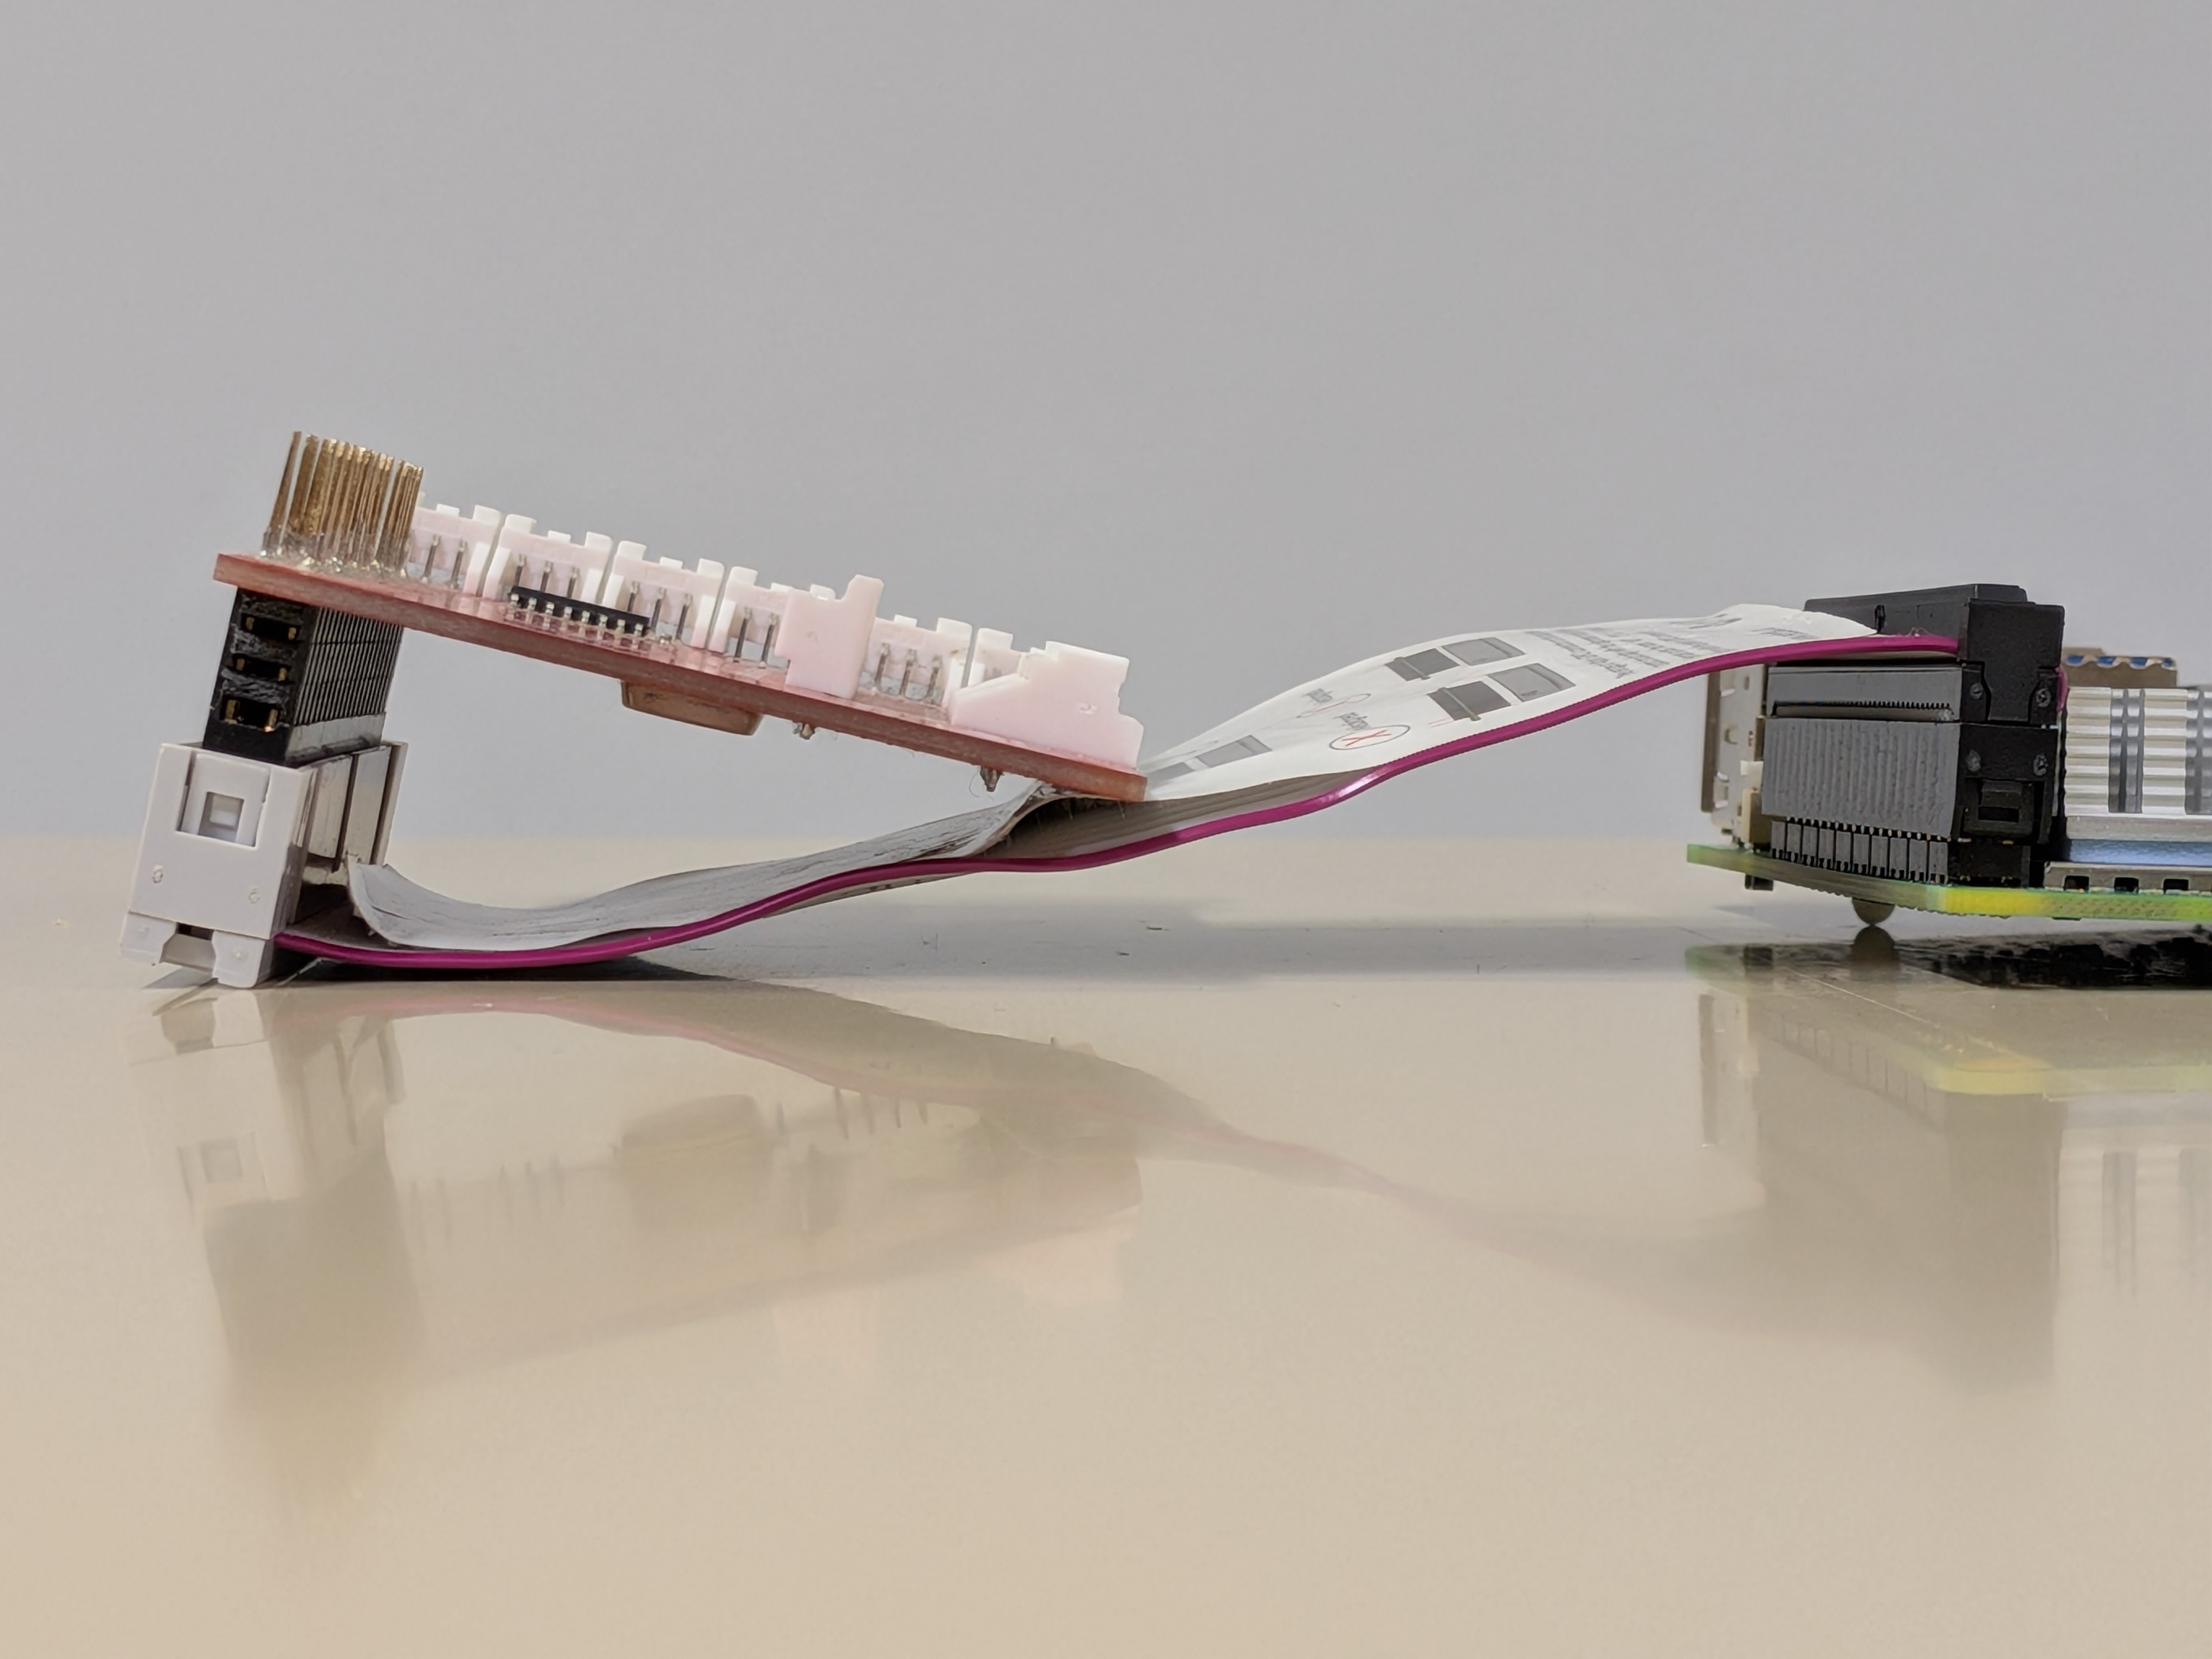
\includegraphics[width=.8\hsize]{../../asset/image/fabo_and_cable_sideview.jpg}
      \caption{FaBoのシールドとケーブルの\ruby{接続}{せつ|ぞく} (横から見た図)}
    \end{figure}
  \end{minipage}
\\
  %\begin{minipage}[b]{0.45\linewidth}
    \begin{figure}[H]
      \centering
      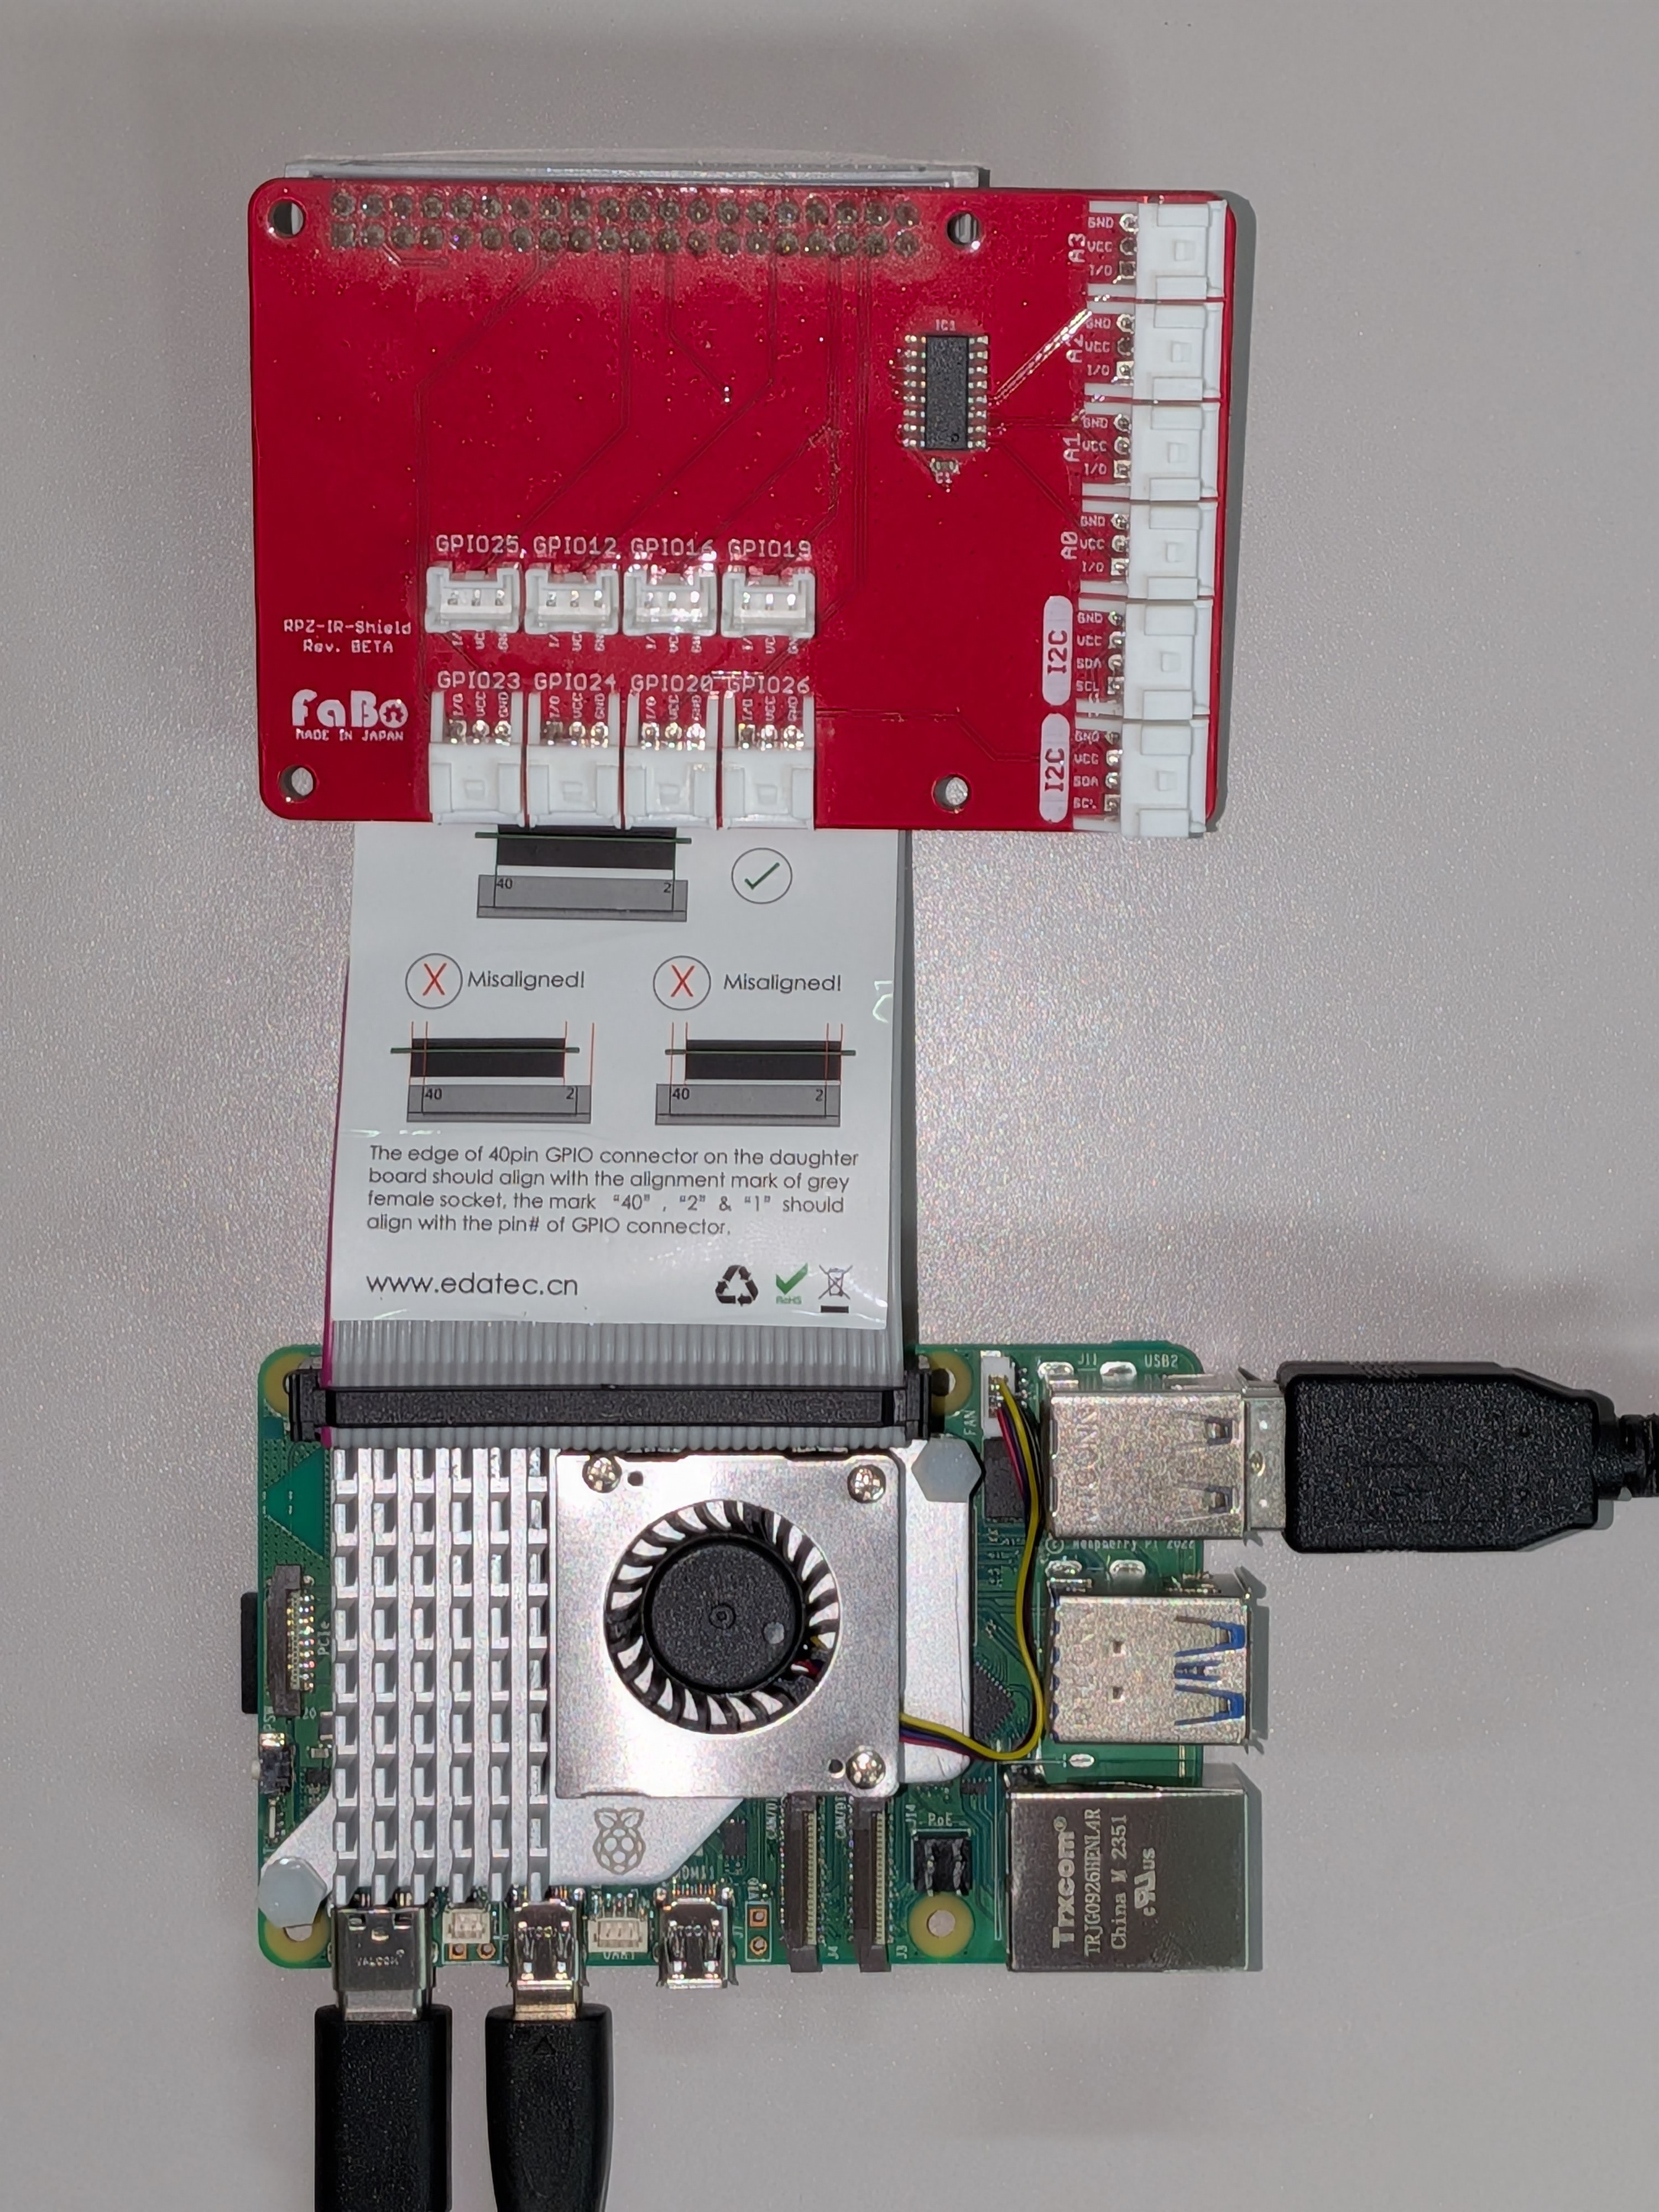
\includegraphics[width=.4\hsize]{../../asset/image/fabo_connected_to_rpi5.jpg}
      \caption{FaBoのシールドとRaspberry Piの\ruby{接続}{せつ|ぞく}\hspace{0pt}}
    \end{figure}
  %\end{minipage}
  \item 同様にして、センサーボードをFaBoのシールドの上につなげます。\\
  \begin{figure}[H]
    \centering
    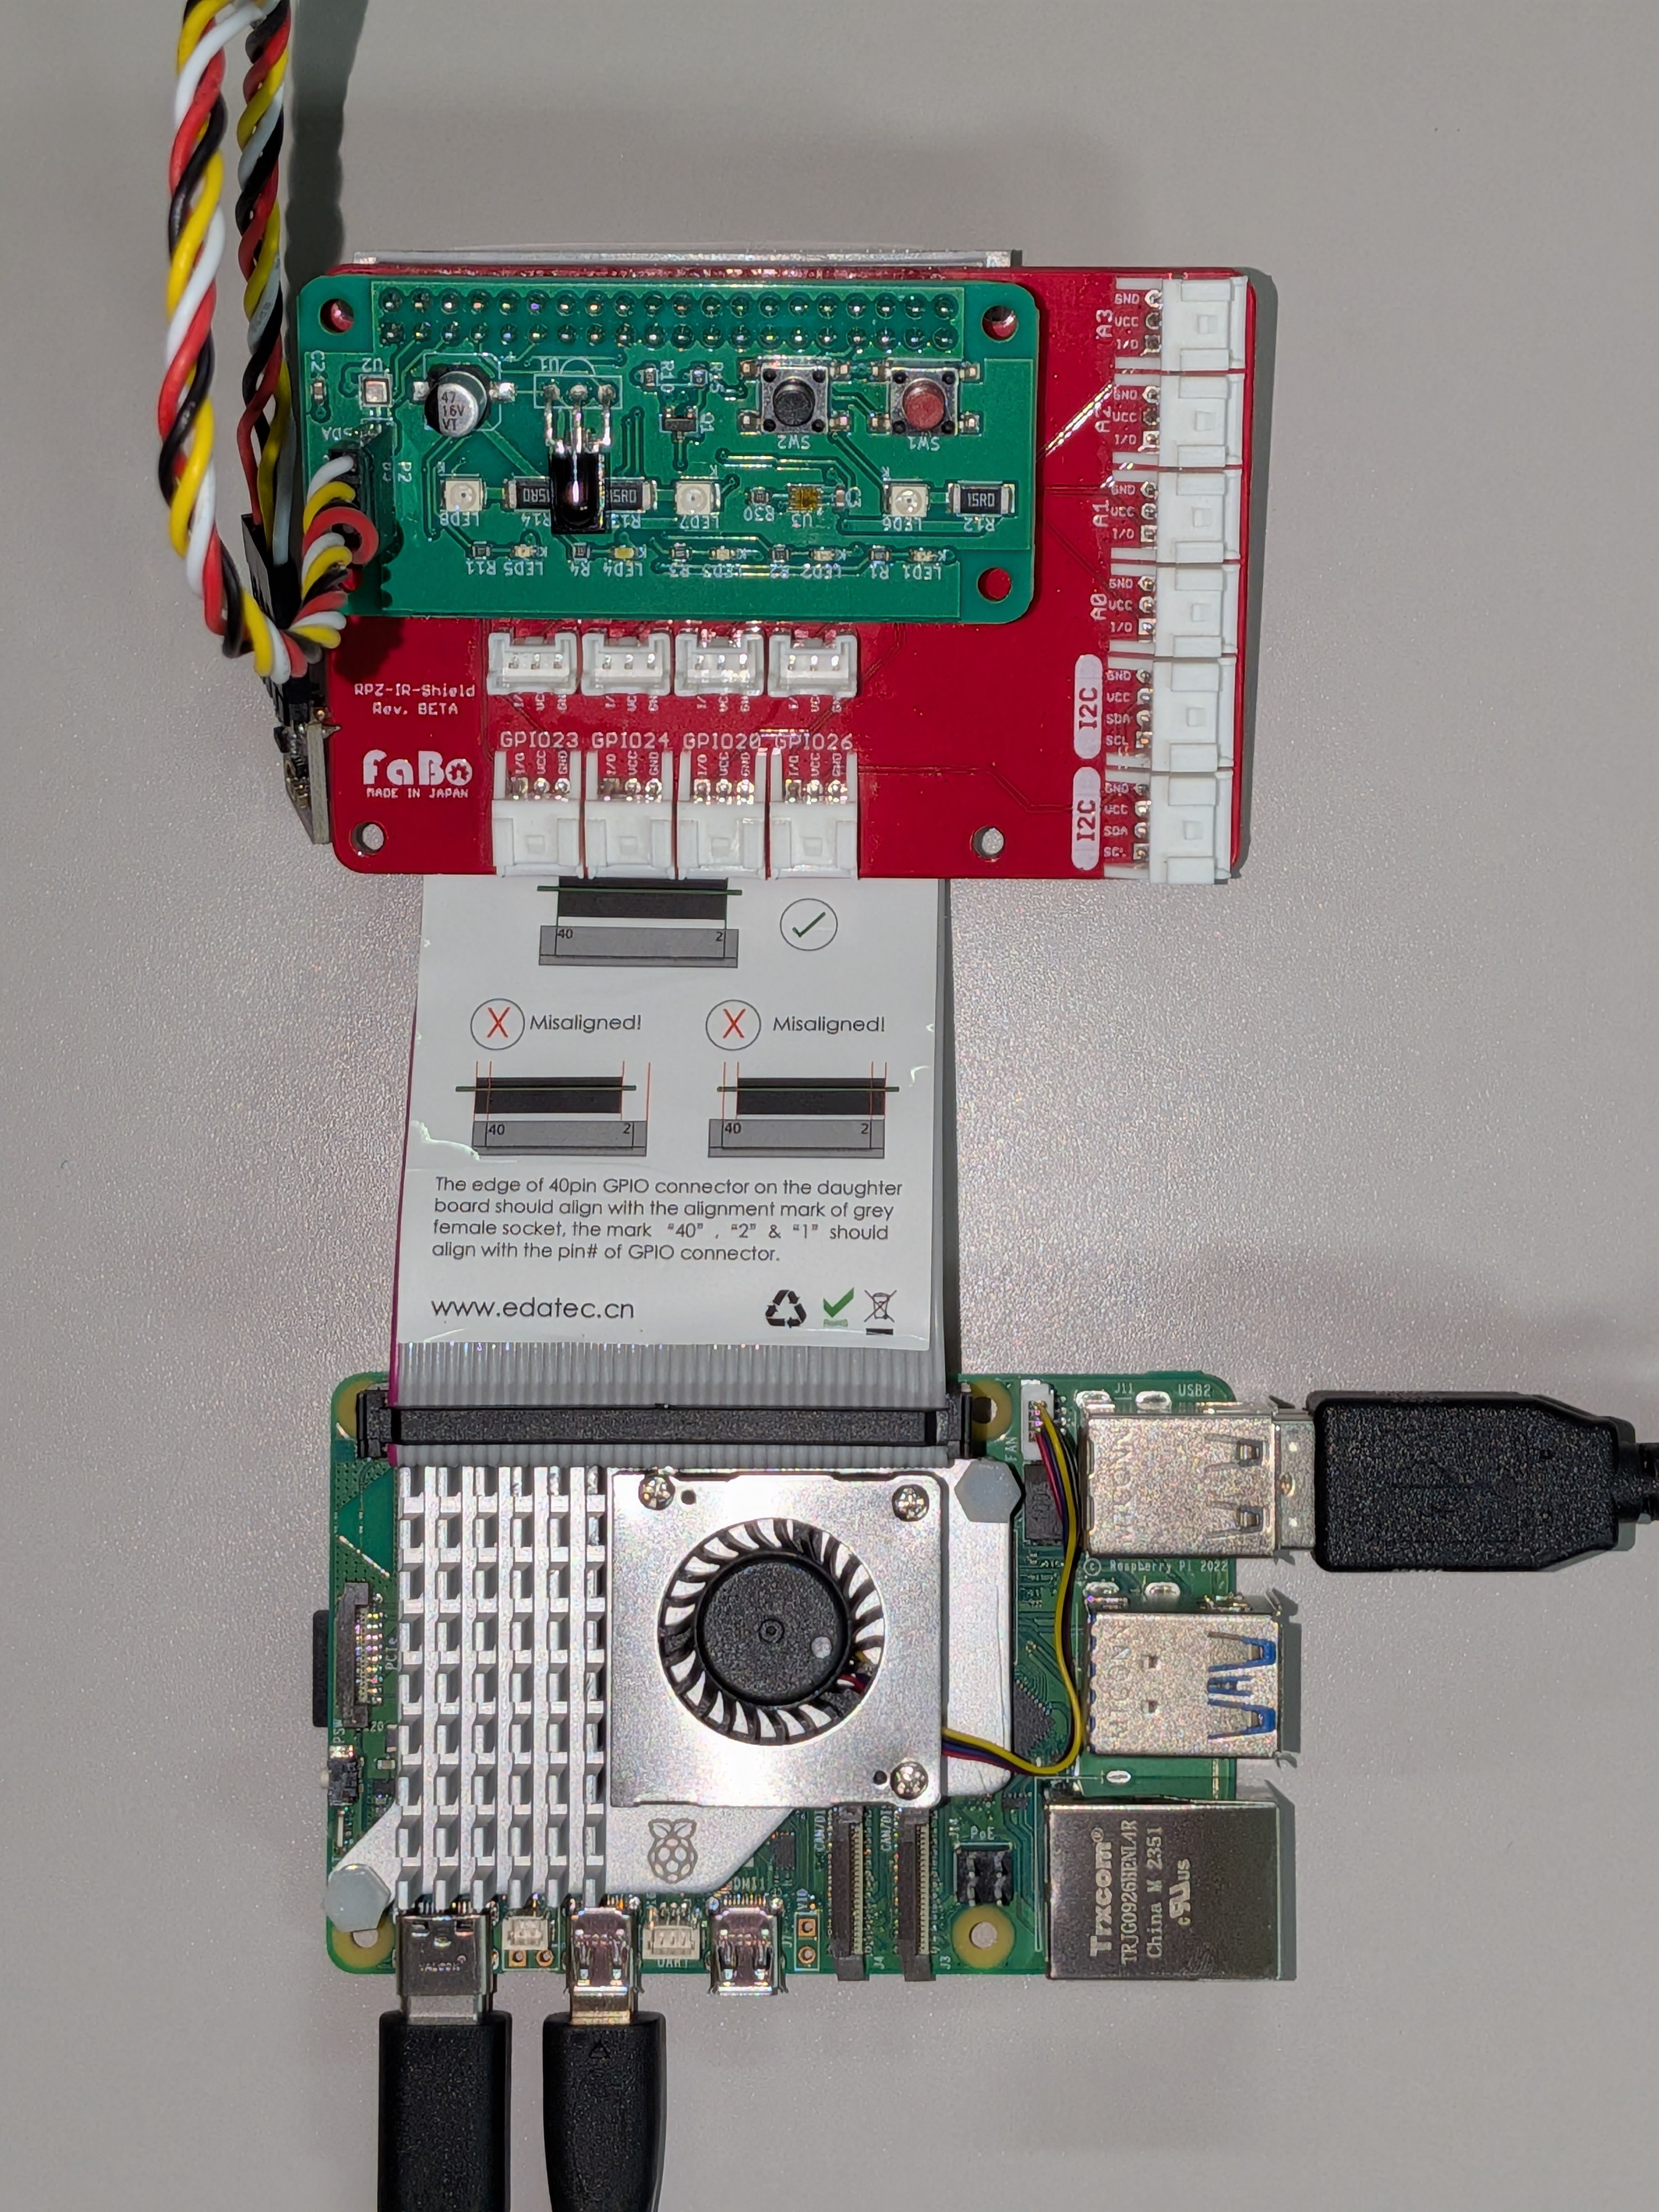
\includegraphics[width=.4\hsize]{../../asset/image/sb_on_fabo_connected_to_rpi5.jpg}
    \caption{センサーボードとFaBoのシールドの\ruby{接続}{せつ|ぞく}\hspace{0pt}}
  \end{figure}
  \item LEDをケーブルとつなげましょう。\ruby{奥}{おく}までコネクタを\ruby{押}{お}しこんでください。\\
  \begin{figure}[H]
    \centering
    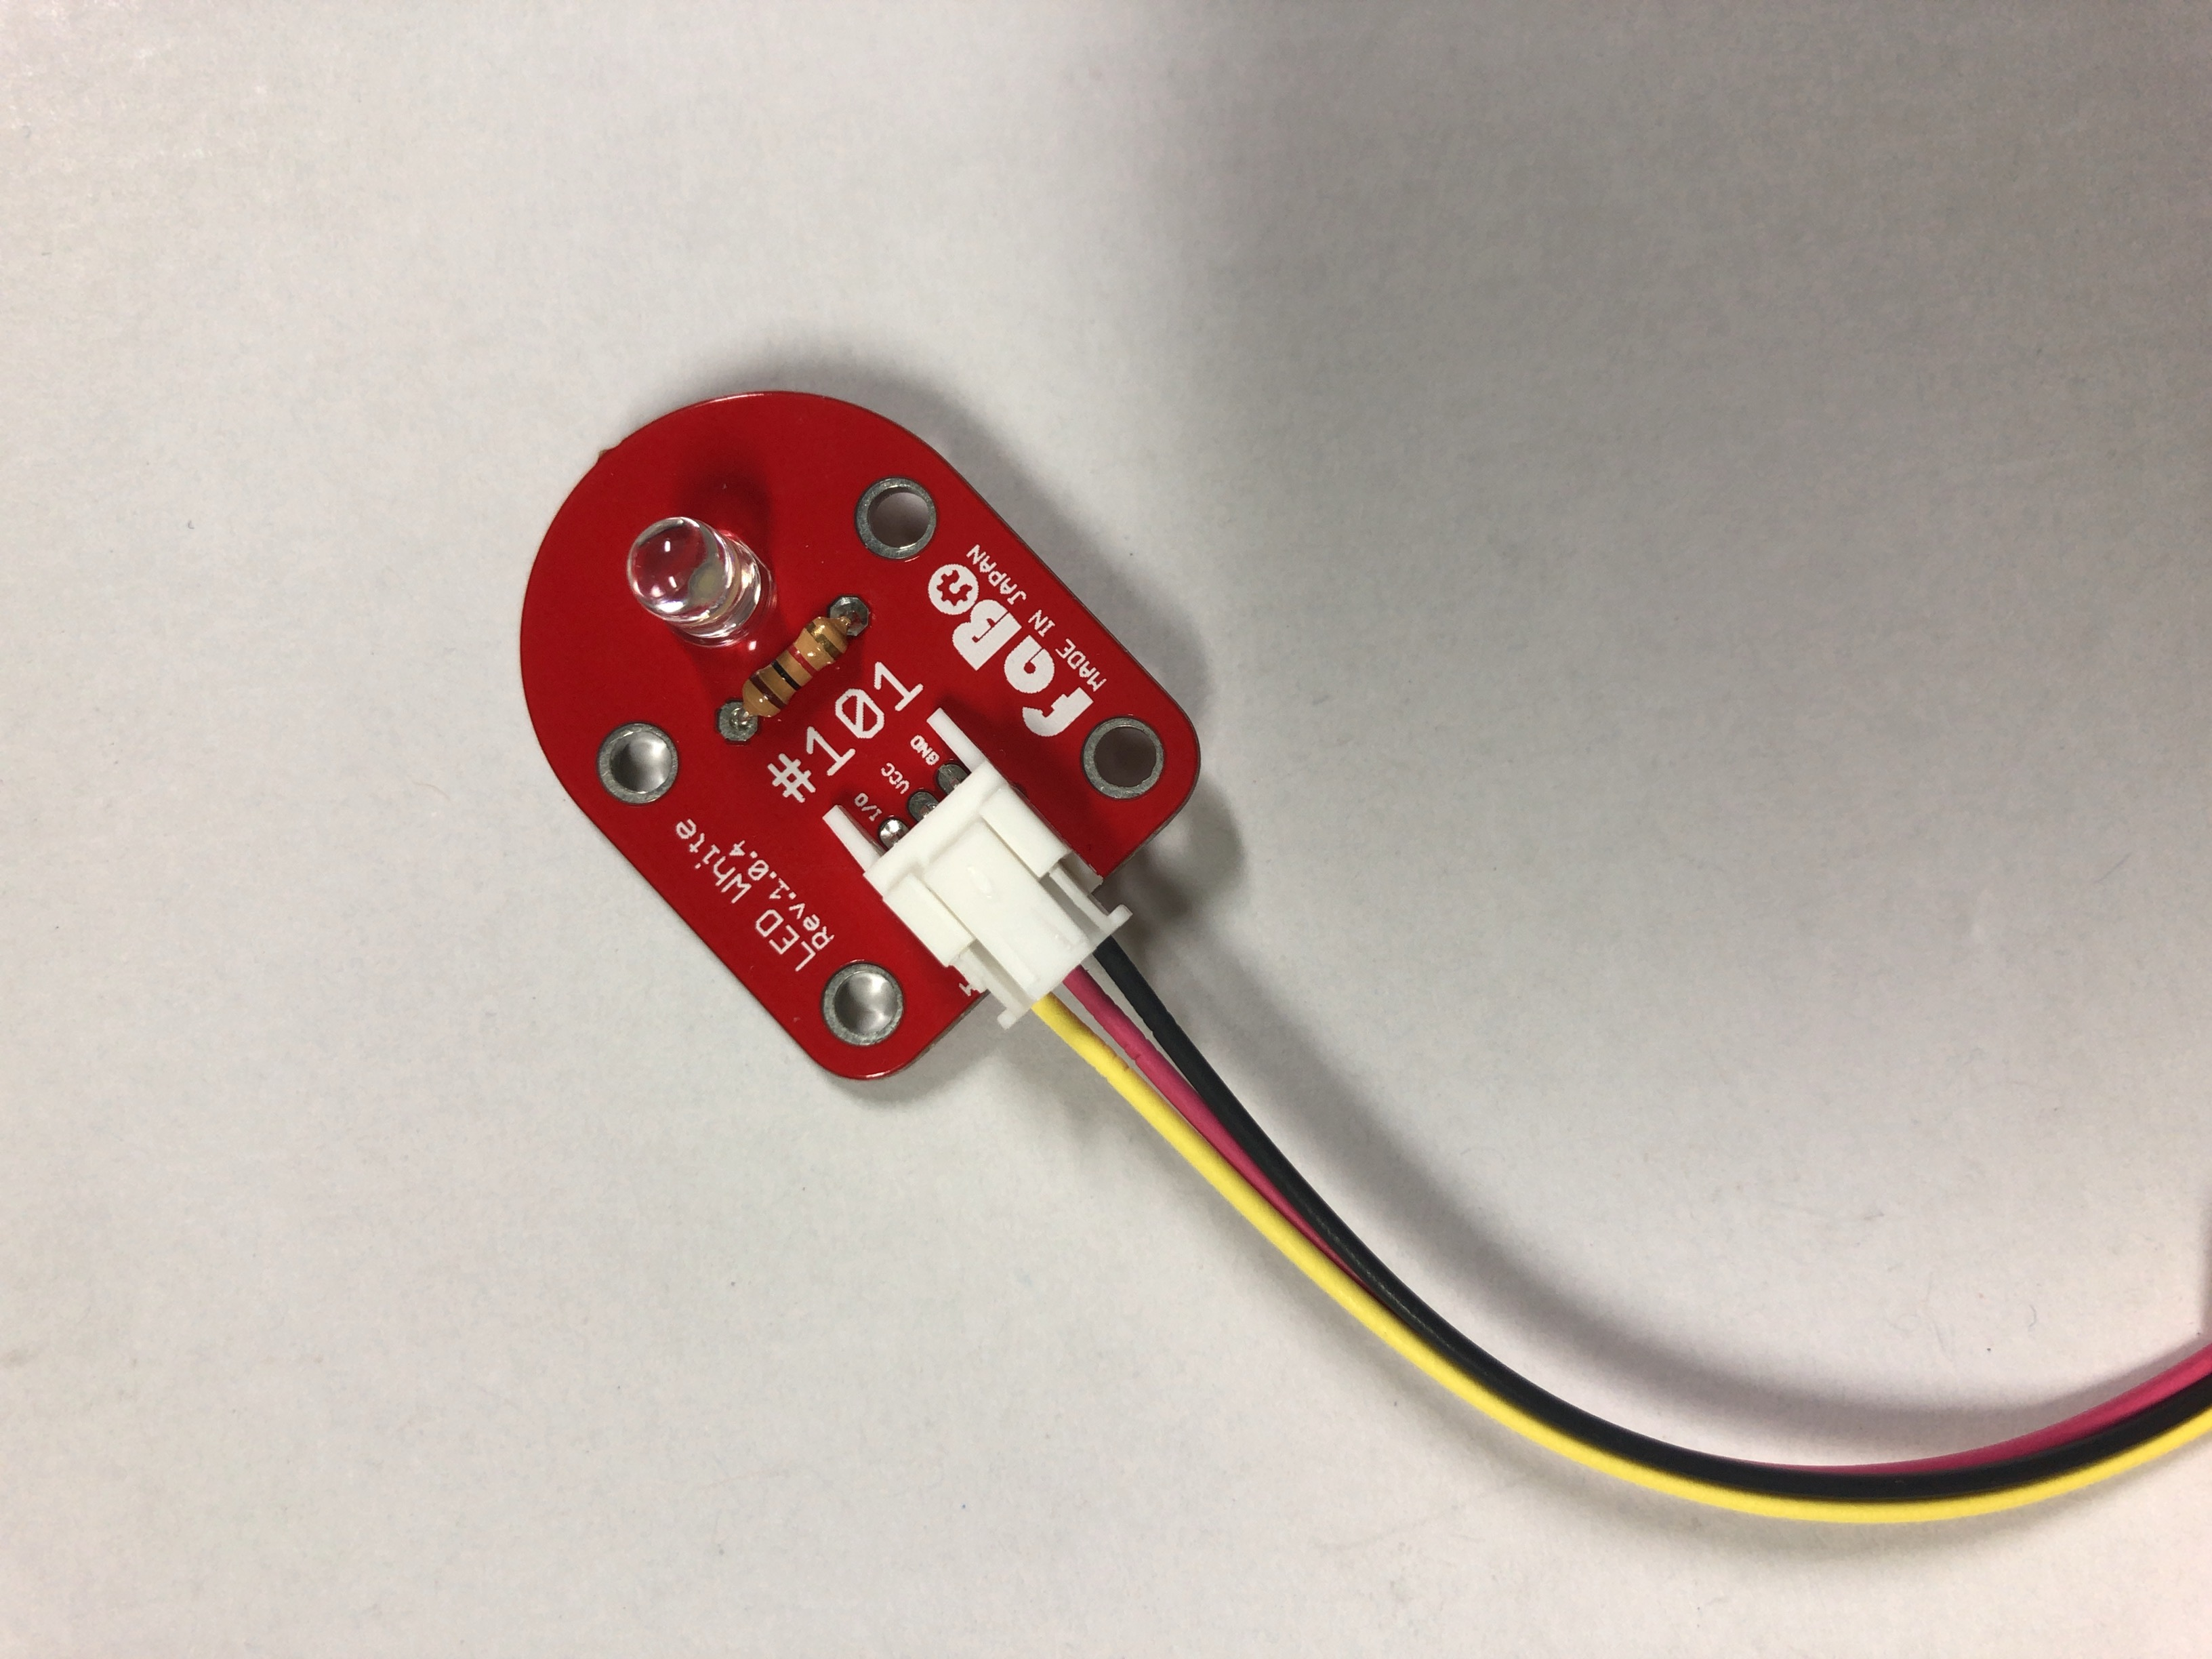
\includegraphics[width=.4\hsize]{../../asset/image/text05-img008.jpg}
    \caption{FaBoのブリックとケーブルの\ruby{接続}{せつ|ぞく}\hspace{0pt}}
  \end{figure}
  \item シールドとケーブルをつなげましょう。今回はGPIO23のところにつなげます。このときも\ruby{奥}{おく}までコネクタを\ruby{押}{お}しこんでください。\\
  \begin{figure}[H]
    \centering
    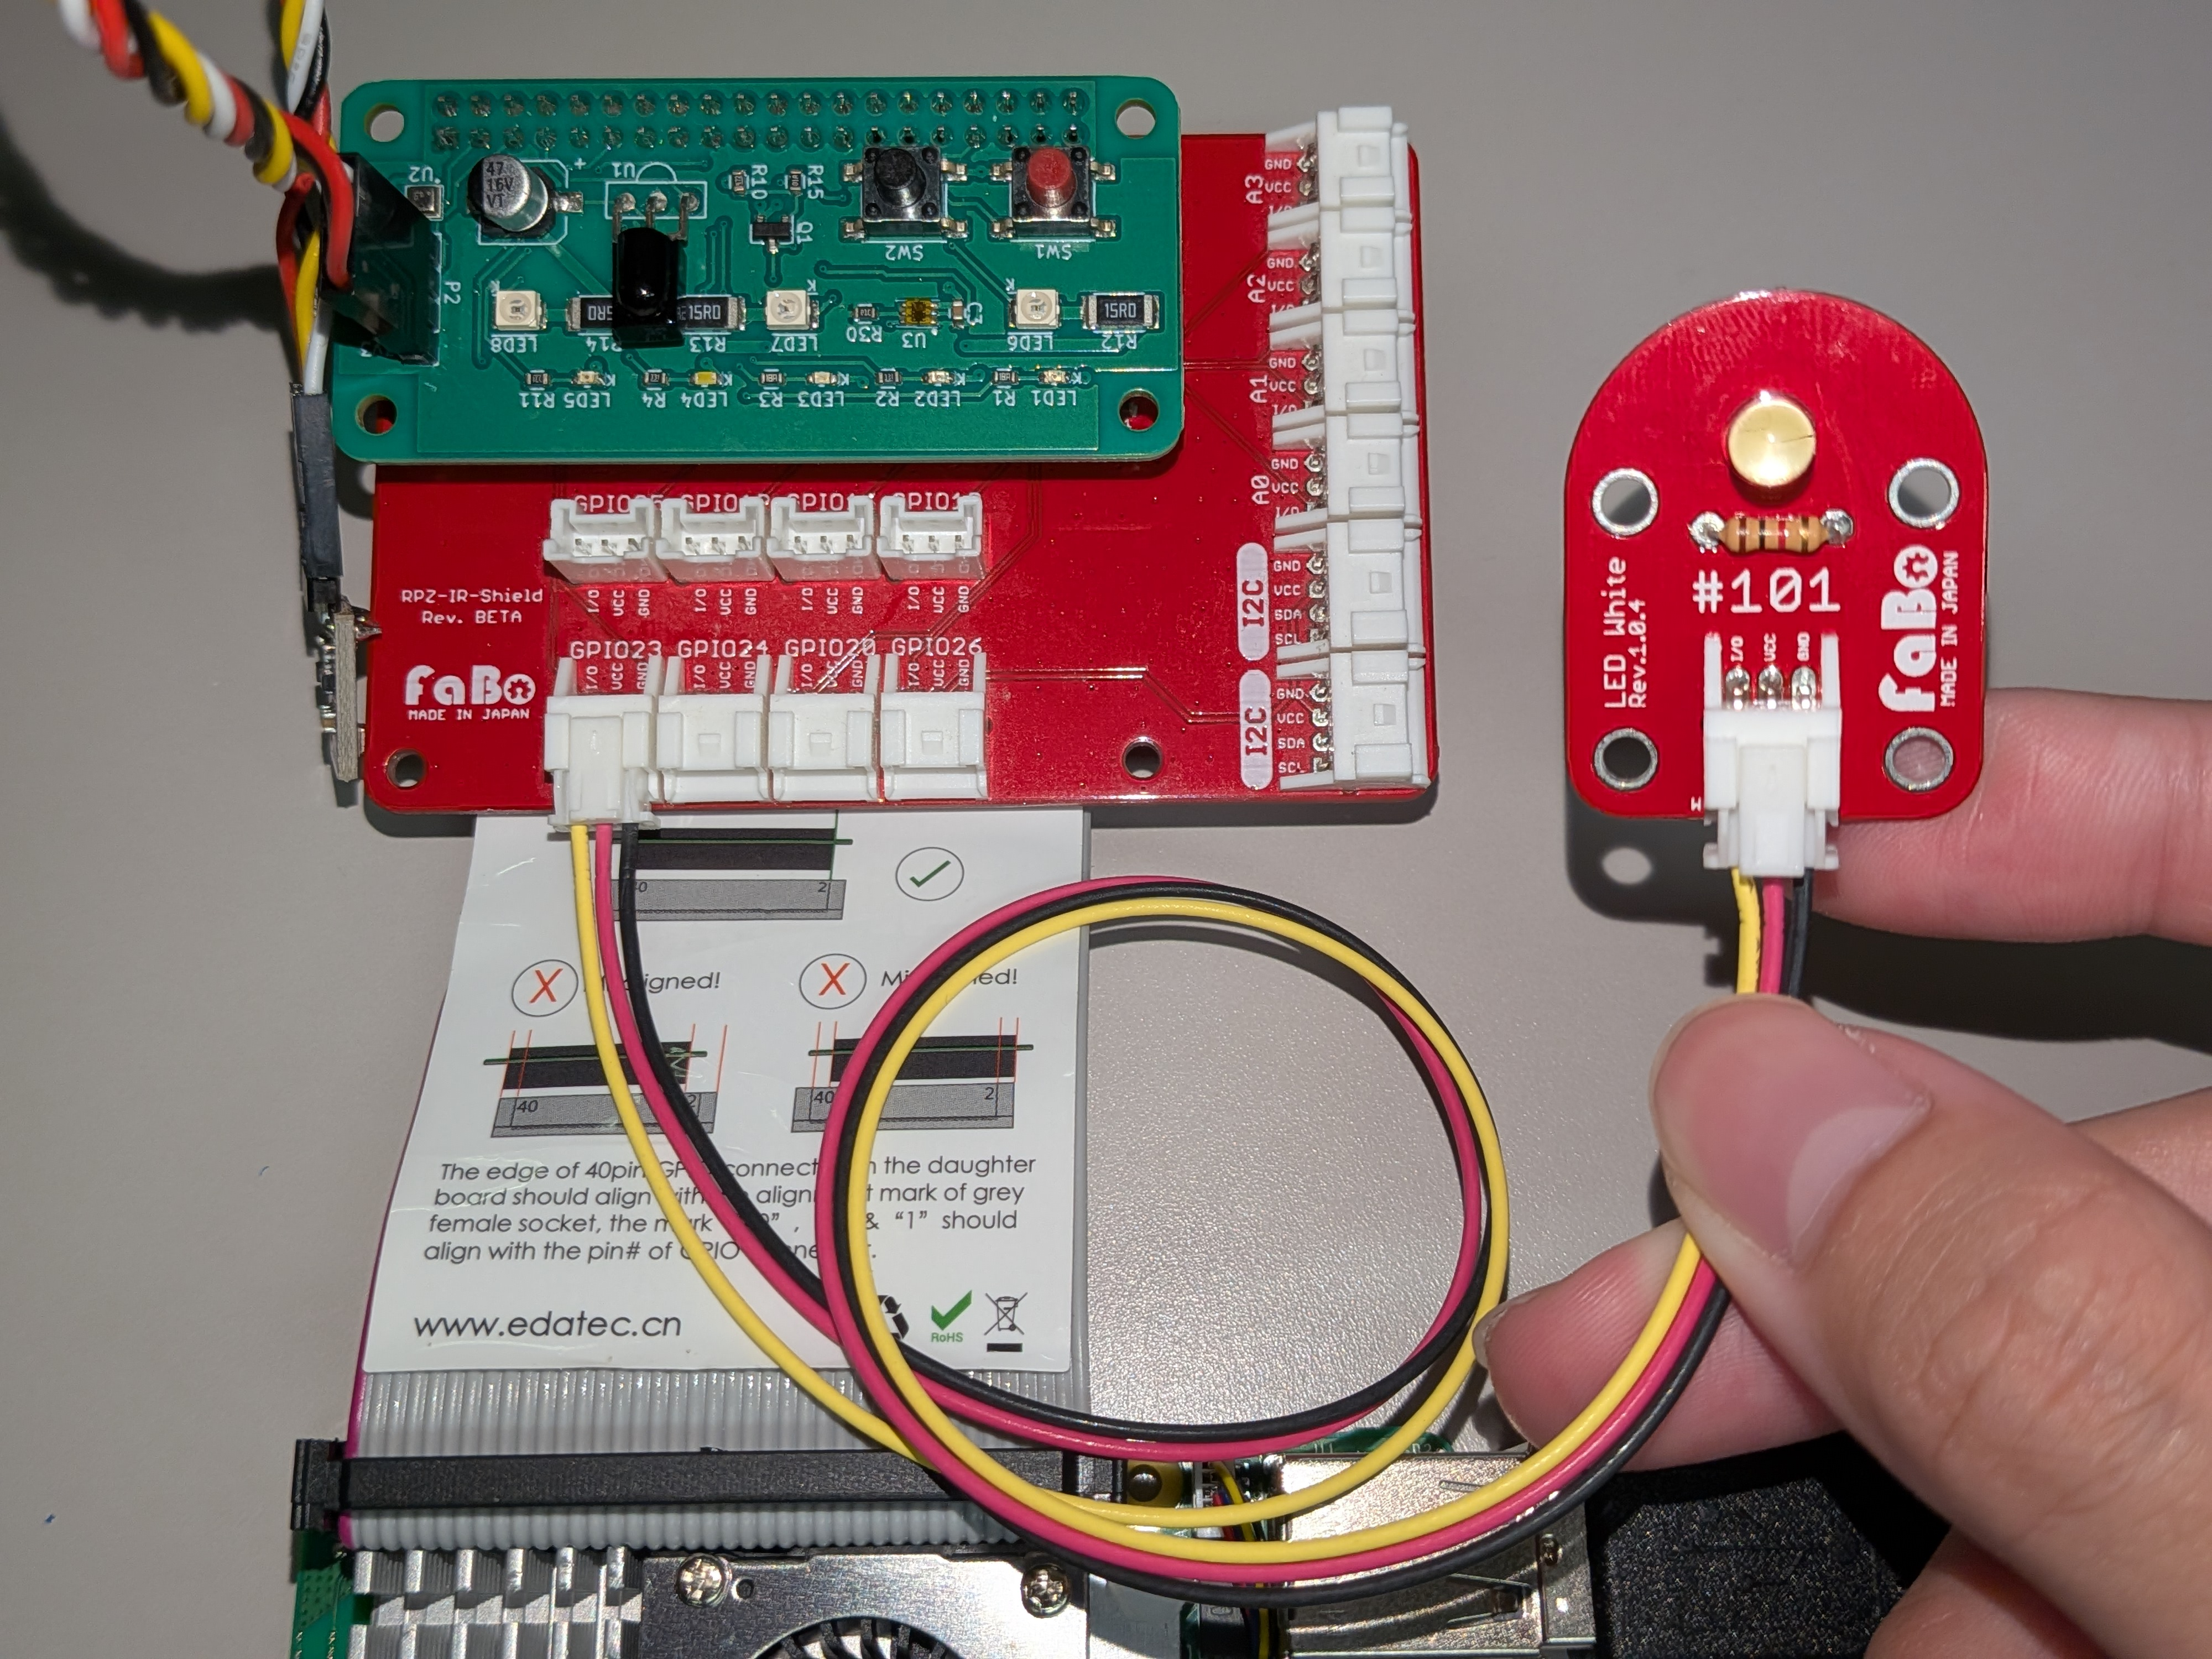
\includegraphics[width=.4\hsize]{../../asset/image/led_brk_on_fabo_with_sb_zoomed.jpg}
    \caption{シールドとケーブルの\ruby{接続}{せつ|ぞく}\hspace{0pt}}
  \end{figure}
  \item ケーブルを外す時は、とがっているツメの部分を\ruby{押}{お}して引き\ruby{抜}{ぬ}いてください。\ruby{抜}{ぬ}けない時や分からない時は周りの先生に聞いてみましょう。\\
  \begin{figure}[H]
    \begin{minipage}[t]{0.45\columnwidth}
      \centering
      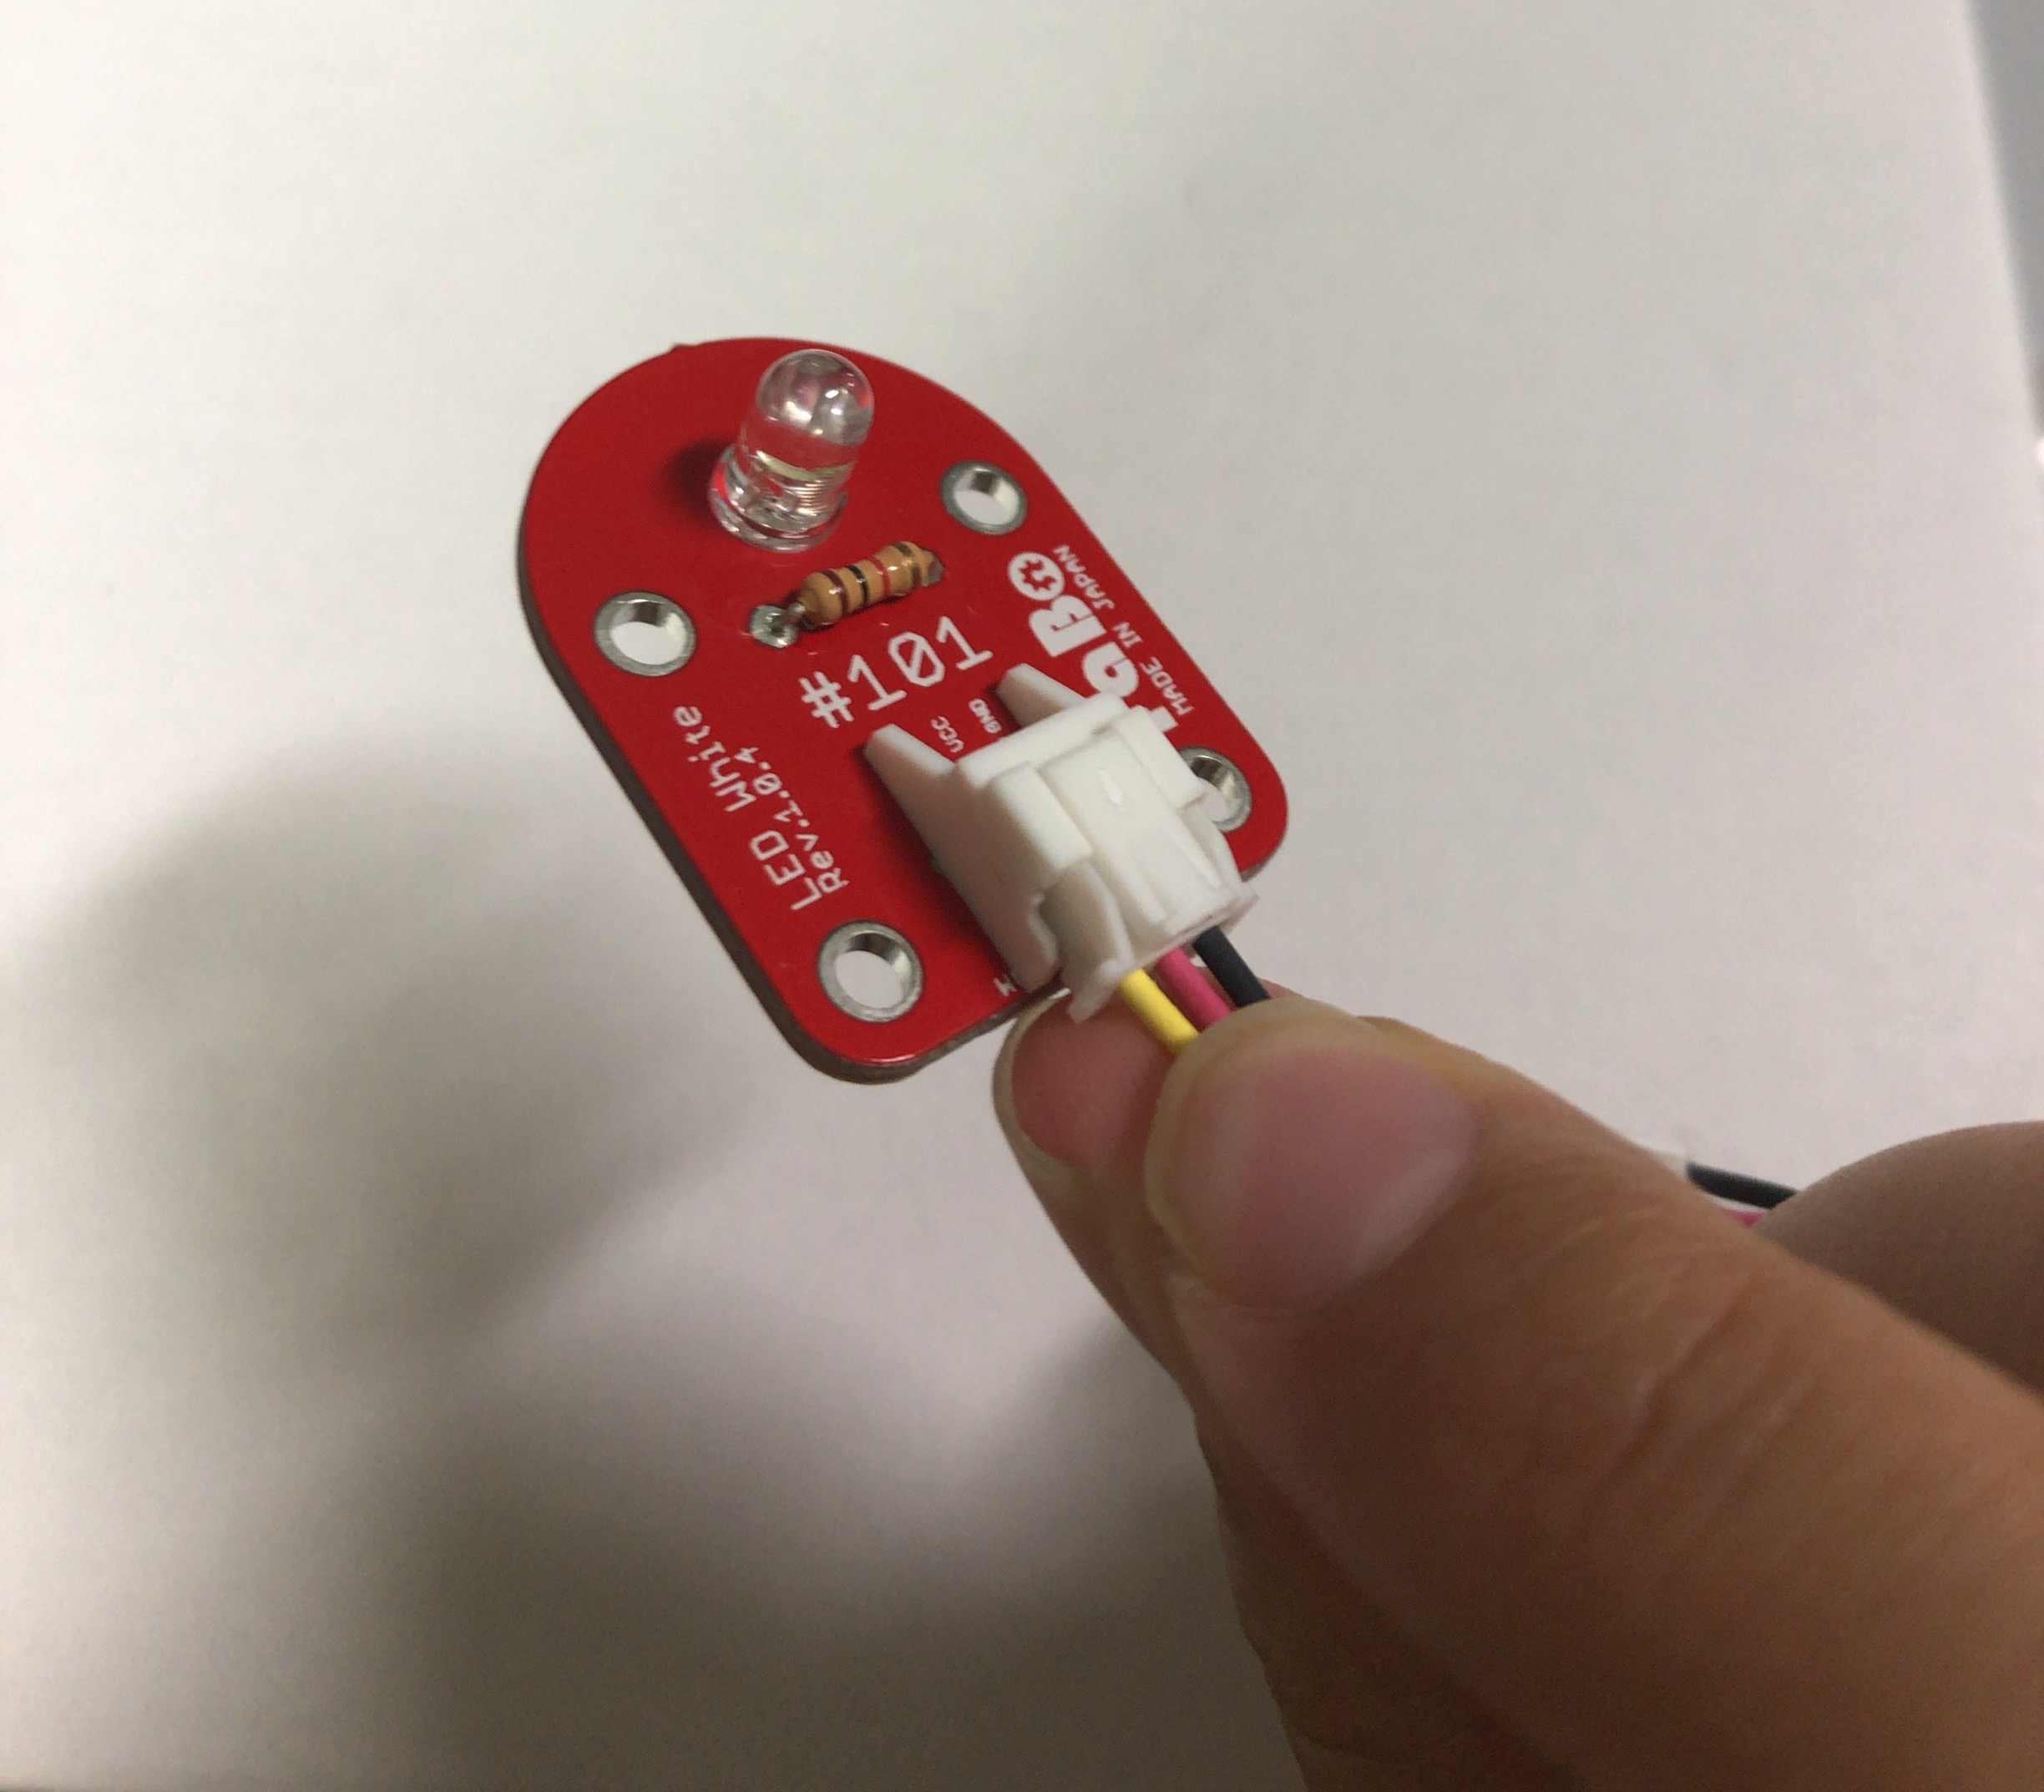
\includegraphics[width=.8\hsize]{../../asset/image/text05-img010.jpg}
      \caption{ケーブルのツメ}
      白い部分の下の方を\ruby{押}{お}します。
    \end{minipage}
    \hspace{0.04\columnwidth} % ここで隙間作成
    \begin{minipage}[t]{0.45\columnwidth}
      \centering
      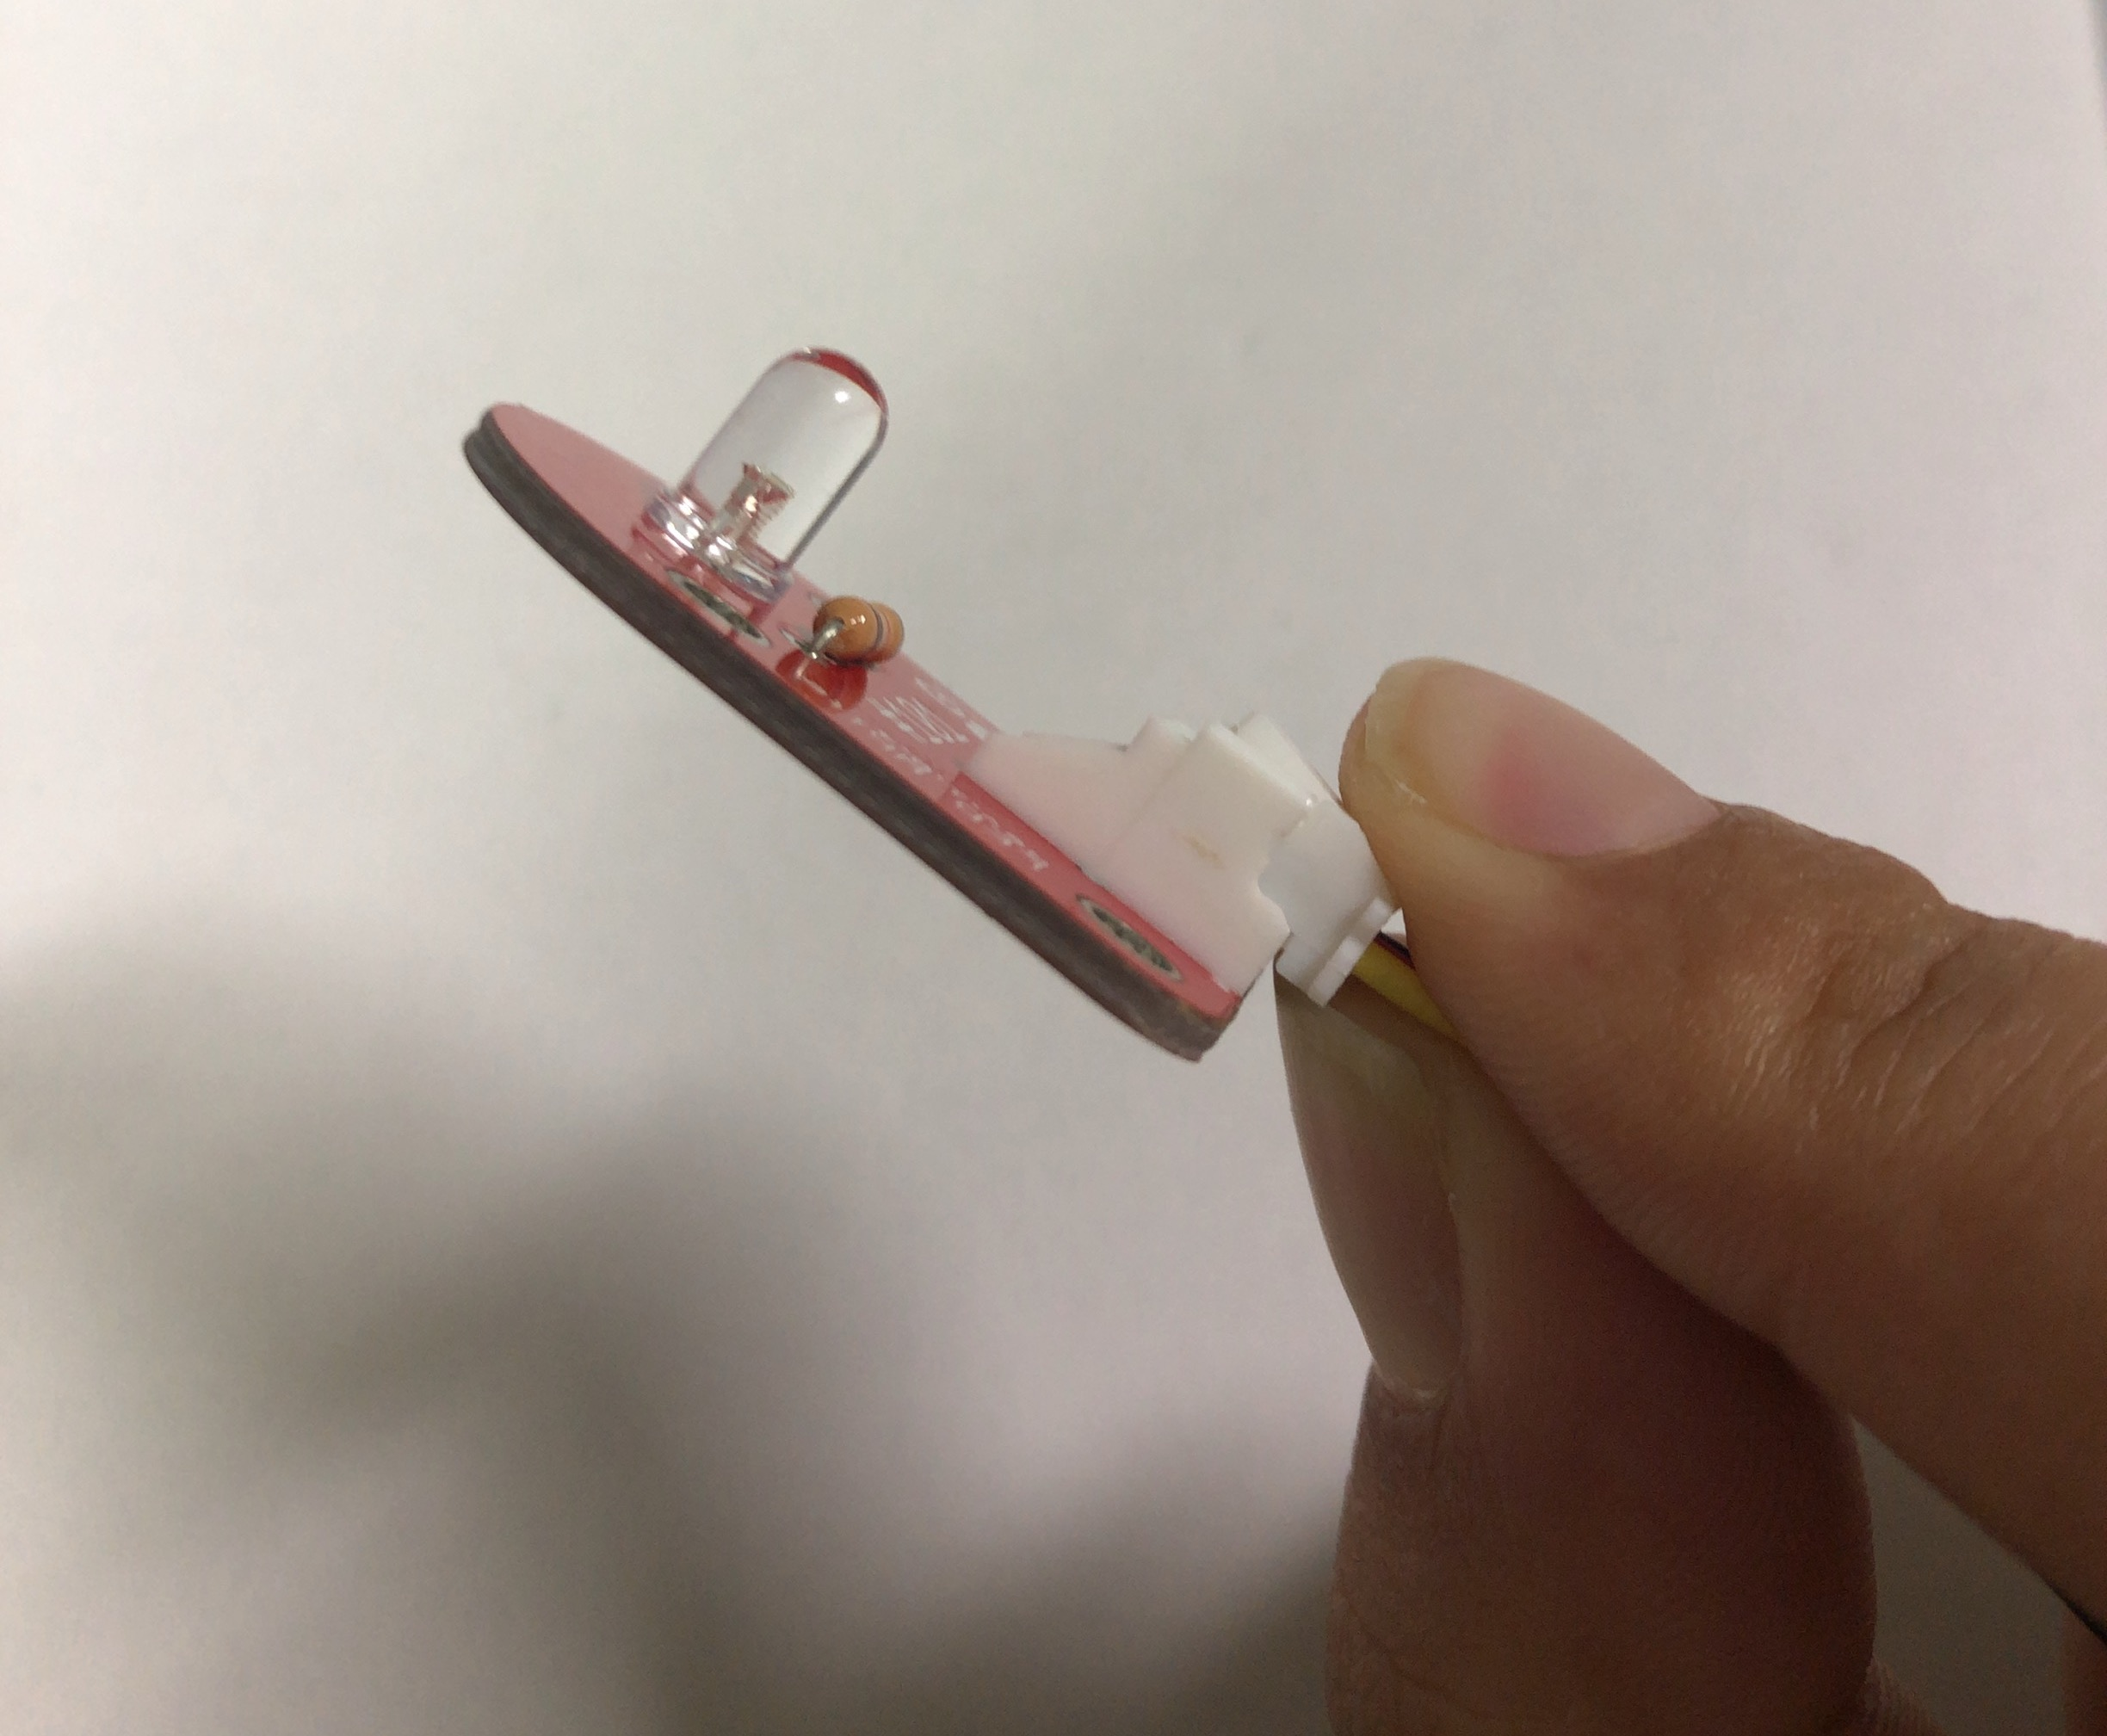
\includegraphics[width=.8\hsize]{../../asset/image/text05-img011.jpg}
      \caption{ケーブルのツメの\ruby{押}{お}し方}
      ツメの部分が少し\ruby{浮}{う}いたら引きぬきましょう。\ruby{抜}{ぬ}けないときは無理に引っぱらず、周りの先生に聞きましょう。
    \end{minipage}
  \end{figure}
  \end{enumerate}


\begin{tcolorbox}[title=\useOmetoi]
\begin{enumerate}
\addex{Raspberry PiとLEDを上記の手順を見ながらつなげてみましょう。}
\end{enumerate}
\end{tcolorbox}















\end{document}
